% ****** Start of file aipsamp.tex ******
%
%   This file is part of the AIP files in the AIP distribution for REVTeX 4.
%   Version 4.1 of REVTeX, October 2009
%
%   Copyright (c) 2009 American Institute of Physics.
%
%   See the AIP README file for restrictions and more information.
%
% TeX'ing this file requires that you have AMS-LaTeX 2.0 installed
% as well as the rest of the prerequisites for REVTeX 4.1
%
% It also requires running BibTeX. The commands are as follows:
%
%  1)  latex  aipsamp
%  2)  bibtex aipsamp
%  3)  latex  aipsamp
%  4)  latex  aipsamp
%
% Use this file as a source of example code for your aip document.
% Use the file aiptemplate.tex as a template for your document.
\documentclass[%
 aip,
%jmp,%
%bmf,%
%sd,%
rsi,%
 amsmath,amssymb,
preprint,%
% reprint,%
%author-year,%
%author-numerical,%
]{revtex4-1}

\usepackage{graphicx}% Include figure files
\usepackage{dcolumn}% Align table columns on decimal point
\usepackage{bm}% bold math
%\usepackage[mathlines]{lineno}% Enable numbering of text and display math
%\linenumbers\relax % Commence numbering lines
%\usepackage{upgreek}

\usepackage[T1]{fontenc}
\usepackage[utf8]{inputenc}
\usepackage[polutonikogreek,english]{babel}
\usepackage{hyperref}
\hypersetup{colorlinks=true,allcolors=blue}
\usepackage[all]{hypcap}

\newcommand{\microsec}{\textgreek{μ}s}
\newcommand{{\usalex}}{smFRET-\textgreek{μ}sALEX}

\begin{document}

\preprint{AIP/123-QED}

\title[48-spot draft]{48-spot single-molecule FRET with alternated excitation}

\author{Antonino Ingargiola}%
 \email{ingargiola.antonino@gmail.com}
\author{Maya Segal}
\affiliation{
Dept. Chemistry and Biochemistry, University of California Los Angeles, USA}
\author{Angelo Gulinatti}
\author{Ivan Rech}
\author{Massimo Ghioni}
\affiliation{%
DEIB, Politecnico di Milano, Italy
}%
\author{Shimon Weiss}%
\author{Xavier Michalet}%
 \email{michalet@chem.ucla.edu}
\affiliation{
Dept. Chemistry and Biochemistry, University of California Los Angeles, USA}


\date{\today}% It is always \today, today,
             %  but any date may be explicitly specified

\begin{abstract}
An article usually includes an abstract, a concise summary of the work
covered at length in the main body of the article. It is used for
secondary publications and for information retrieval purposes.
%
Valid PACS numbers may be entered using the \verb+\pacs{#1}+ command.
\end{abstract}

\pacs{Valid PACS appear here}% PACS, the Physics and Astronomy
                             % Classification Scheme.
\keywords{Suggested keywords}%Use showkeys class option if keyword
                              %display desired
\maketitle

\section{Introduction} \label{sec:intro}

Among the solution-based single-molecule FRET
(smFRET) methods, \emph{microsecond alternated excitation}
({\usalex}) is one of the most powerful.
In {\usalex} two exciting lasers are alternated with a period of a
few tens of {\microsec} and the fluorescent emission is detected in two
spectral bands (donor and acceptor, or D and A) by two separate
detectors. Using two alternating lasers for excitation, a family of
techniques dubbed ALEX\cite{Kapanidis_2005}, allows separating singly- from
doubly-labeled species, greatly extending the range of subpopulations
that is possible to resolve in a given sample. As an example, dual-laser
excitation allows separating D-only from zero or low FRET species that would
be indistinguishable with only a single excitation laser.

Single-molecule FRET Periodic Acceptor Excitation (smFRET-PAX)
\cite{Doose_2007} is a technique closely related to {\usalex},
where the D laser is constantly on and the A laser is alternated. This
approach allows simplifying the optical setup while maintaining the same
advantages of {\usalex}, namely the ability to resolve species based
on the number of attached dyes.

\section{Setup description}\label{setup-description}

\begin{figure*}
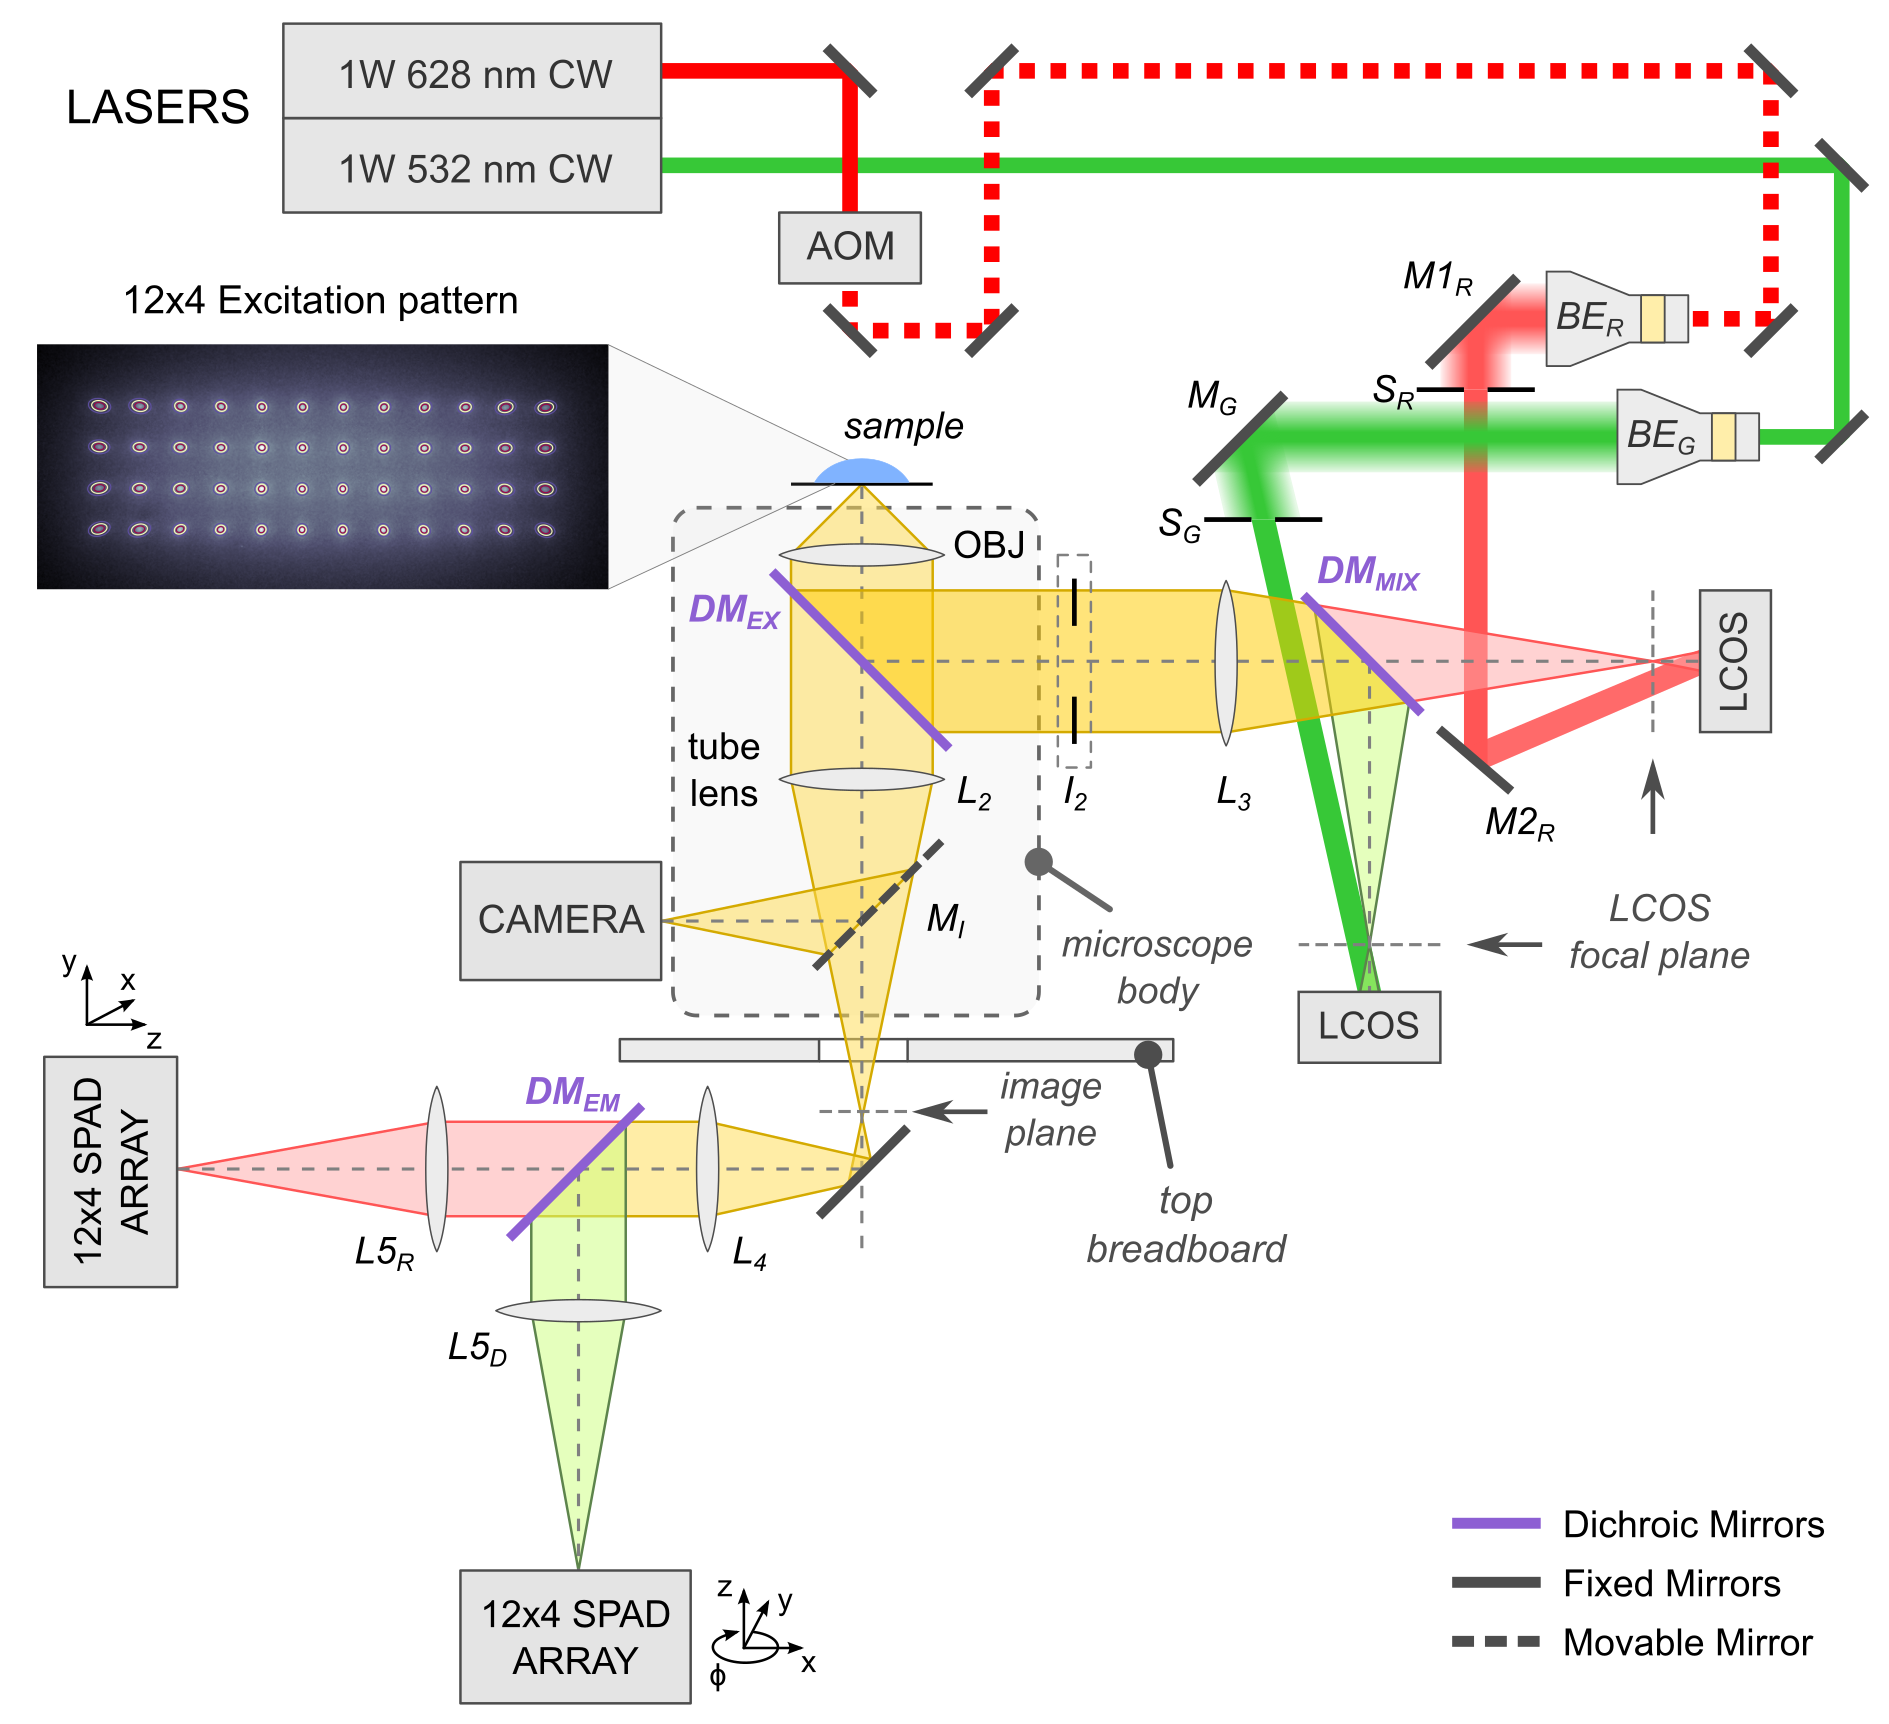
\includegraphics[width=0.7\textwidth]{figures/design_multispot_LCOS_camera_SPAD}
\caption{{\label{fig:setup} Schematic of the 48-spot smFRET-PAX setup.}}
\end{figure*}

The setup (Fig. \ref{fig:setup}) comprises two excitation CW lasers at
532~nm and 628~nm (2RU-VFL-Series, MPB Communications Inc., QC, Canada).
For each laser, a half-waveplate and polarizing beam splitter are used
for polarization and intensity control, as the polarization orientation
needs to be aligned along the direction required by the LCOS-SLM. The
628 nm laser is directed through an acousto-optical modulator (P/N 48058
PCAOM, electronics: P/N 64048-80-.1-4CH-5M, Neos Technology, Melbourne,
FL, USA) used for {\microsec} time-scale modulation, while the 532~nm
laser is unmodulated.
Each laser goes through a first beam expander (Keplerian
telescope, doublet lenses: 50~mm and 250~mm focal lengths). Two periscopes
bring the beams to a raised optical breadboard where a microscope body
(X71, Olympus Corporation, Japan) is fixed with its bottom port sitting
over a circular aperture. Past the periscope, each beam goes through a
second adjustable beam expander (3X, P/N 59-131, Edmund Optics Inc.).
The red laser is reflected off mirrors $M1_R$ and
$M2_R$ and phase-modulated by the ``red'' LCOS-SLM (P/N
X10468-07, Hamamatzu, Japan), before passing through the dichroic mirror
$D_{MIX}$. The green laser is reflected off $M3$,
phase-modulated by the ``green'' LCOS-SLM (P/N X10468-01, Hamamatzu),
and combines with the red excitation via the dichroic mirror
$D_{MIX}$ (T550LPXR, Chroma Technology Corp, VT, USA). Both
beams are recollimated by the $L3$ lens (f=250mm,
AC508-250-A, Thorlabs) and focused into the sample by an high-NA
objective lens (UAPOPlan 60x, NA 1.2, Olympus) after being reflected off
the excitation dichroic mirror $DM_{EX}$ (Brightline
FF545/650-Di01, Semrock Inc., NY, USA). The excitation pattern forms a
dual-color 12x4 array of spots into the sample matching the geometry of
the two SPAD arrays. The fluorescence emission is collected by the same
objective lens, passes through the excitation dichroic
$DM_{EX}$ and is focused by the microscope tube lens either on
the side or the bottom port of the microscope. The side port mounts an
sCMOS camera (Grasshopper3 GS3-U3-23S6M-C, FLIR Integrated Imaging
Solutions Inc., BC, Canada) used during alignment while the bottom port
redirects the beams toward the emission path. Here, a relay lens
$L4$ (f=100mm, AC254-100-A, Thorlabs) recollimates the
image and sends it to an emission dichroic mirror $D_{EM}$
(Brightline Di02-R635, Semrock), which splits the signal into a donor
(D) and acceptor (A) spectral bands. The D path goes through a band-pass
filter (Brightline FF01-582/75, Semrock) which removes residual 628~nm
laser leakage and helps suppressing any Raman scattering from the 532~nm
laser. Both D and A paths are refocused by lenses $L5_D$ /
$L5_A$ (f=150~mm, AC254-150-A, Thorlabs) on two 48-pixels
SPAD arrays\cite{Gulinatti_2013} (denoted as donor and acceptor SPAD in the
following).

Both SPAD arrays are place on 3-axis micro-positioners. The directions
orthogonal to the optical axis (X-Y) are controlled by piezo actuators
(actuators: Newport 8302; drivers: Newport 8752 \& 8753; Newport
Corporation, Irvine, CA, USA). The third axis (Z) has manual actuators
since the requirements on the Z directions are much less stringent than
for the X-Y directions. The donor SPAD array has an additional stage for
rotation about the optical axis, used to match the relative orientation
of the SPAD arrays.

Each SPAD arrays is equipped with an USB 2.0 connection for time-binned
counting and humidity control. In addition, a standard SCSI connector
includes 48 independent outputs providing a pulse for every detected
photon in each pixel\cite{Gulinatti_2013}. The two SCSI ports are fed
through a custom adapter to an FPGA-based acquisition board (FPGA board:
PXI-7813R, rack: PXI-1000B, National Instruments, Austin, TX) which
performs timestamping with 12.5~ns resolution in parallel on the 96
channels (task implemented in LabVIEW 2011 using the FPGA Toolkit). The
board transfers the data asynchronously to a host PC via an MXI-4 link
to a custom acquisition program written in LabVIEW 2011 (MXI-4 link:
rack board PXI-8331; PC board PCI-8331, National Instruments). The
acquisition program also controls the red laser alternation using a
pulse generation board (PXI-6602, National Instruments), whose clock is
synchronized with the timestamping FPGA board (PXI-7813R) through the
common rack (PXI-1000B).

In addition to the aforementioned acquisition program, the host computer
runs a second LabVIEW 2011 programs controlling the phase pattern on the
two LCOS-SLM. During alignment the acquisition program communicates with
the LCOS-control programs to scan the positions of the LCOS pattern and
assess position of the SPAD arrays (see section XXX).

The raw binary data is saved together with a text-based metadata file
containing measurement details that are used to create the final
Photon-HDF5 file\cite{Ingargiola_2016a}. Once the measurement is saved on the
host PC, the raw data is immediately transferred to a linux-based
workstation via 1~Gb Ethernet link. The second workstation automatically
performs conversion to Photon-HDF5 and data analysis, leaving the host
PC available for acquiring the next set of data.

\section{Laser alignment}\label{sec:laseralign}

Each for the two lasers need to be aligned in order
to ensure (a) the maximum uniformity between spots intensities (b) the
minimal aberrations across the patterns. To achieve (a) the Gaussian
laser beam is expanded so that only the central part of the beam covers
the excitation pattern (which has a maximum extension of 5mm). To ensure
(b), the geometrical center of the pattern needs to be placed on the
optical axis.

In addition, (c) the excitation pattern of the two laser need to be
aligned so that, for each spot, there is a maximum overlap between D
and A excitation volumes.

\subsection{Individual laser
alignment}

The 3x monolithic beam expanders have an adjustment ring used to adjust
the beam collimation. A simple way to ensure beam collimation is sending
the beam into the microscope through the excitation dichroic, removing
the external recollimation lens $L3$ and the objective
lens, while placing a mirror on the sample holder and using the LCSO-SLM
as a mirror (i.e.~with a constant phase pattern). Using the camera on
the microscope output port, we adjust the collimation until a tight spot
is formed. After adjusting the collimation, each beam needs to be
aligned so that the peak intensity is at the center of the optical axis.
To this end, without the recollimating lens $L3$, an iris
$I2$ is placed before the beam enters the microscope side
port. Using an aperture of 1-2 mm, only a narrow beamlet goes through
the objective and generates a spot from the cover-glass reflection. Only
when the input beam is parallel to the optical axis, the spot is in the
center of the field of view, assumed to be on cross-hair center in the
microscope's eyepiece. In order to make the input beams parallel to the
optical axis, the last mirrors before the microscope is adjusted
($M2_R$ for the red and $DM_{MIX}$ for the green
laser). Defocusing the spot, we obtain symmetrical concentric patterns
only if the input beamlet intersects with the optical axis at the back
aperture of the objective lens. Since the direction is already fixed, we
move the $I2$ iris to obtain the most radially-symmetric
defocused pattern. In this way the beamlet that goes through
$I2$ coincides with the microscope optical axis. The last
steps is translating laterally the input beams (without changing the
incidence angle) in order to place the intensity peak on the iris
center. Alignment of beam direction and iris need to be repeated a until
convergence. After that, both beams are (to a good approximation)
parallel and concentric with the optical axis. When placing
$L3$ a spot is formed at a different focus position.
$L3$ can be aligned assuring that this new spot is a the
same position of the spot obtained without $L3$.

\subsection{Coalignment of Green and Red
patterns}

Starting with the green LCOS-SLM, we project a multispot pattern into a
high concentration solution of dyes (100~nM - 1\textgreek{μ}M) used for alignment.
Using a square grid of spots with an odd number of spot per side
(i.e.~9x9) ensures that one spot is at the center of the pattern. The
camera on the side-port detects an image of the pattern. The centering
of the pattern with respect to the optical axis can be assessed from the
amount of geometrical aberrations in the lateral spots. We center the
excitation pattern by rigidly translating the pattern on the LCOS-SLM so
that geometrical aberrations are roughly equivalent on the four sides.
Next, we perform a 2-D Gaussian fitting of each spot, and from the
distribution of sigmas and rotation of each Gaussian we estimate a more
accurate position of the the optical axis (analysis performed with
notebook XXX). This step may be repeated a few times until convergence.
From this point on, the X-Y positions of the green LCOS-SLM is not
changed anymore and its center becomes a reference for the optical axis
position.

Next, we activate the red LCOS-SLM and project a multispot pattern
excited by the 628~nm laser. Using the camera we align the red pattern to
the green one used as reference. A first rough adjustment of red
LCOS-SLM pattern is manually performed by looking at the emission
pattern on the live camera display. Then, the center position red
LCOS-SLM pattern is finely tuned by fitting the spot positions in the
green and red images (Fig. \ref{fig:patternfit}), taken separately (the
analysis notebook can be found in
\href{https://github.com/multispot-software}{multispot-software}).

Finally, in order to reduce the background due to unmodulated light, two
custom-made rectangular slits (aluminum with black finish) are added in
the path before each LCOS. The slits are aligned to illuminate only the
12x4 pattern (\(\pm\)1~mm) on the LCOS-SLM.

\begin{figure}
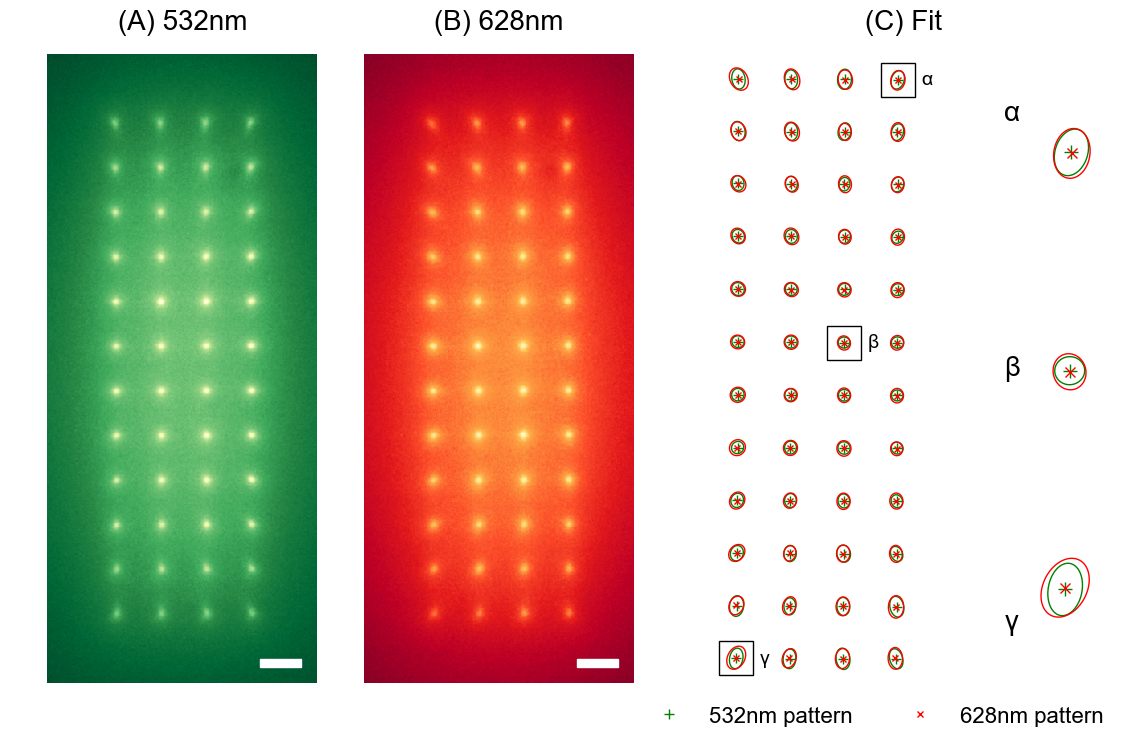
\includegraphics[width=\columnwidth]{{figures/2017-04-28_conf9_G_conf14_R_green_red_pattern_and_fit}}
\caption{{\label{fig:patternfit}
The 12x4 multispot pattern for green (A) and red (B)
excitation and Gaussian fit of the spots (C). The pattern is acquired by
a camera on the microscope side port using a solution of ATTO550 and
ATTO647N at high concentration (\(\sim\)100~nM). Emission due
to 532~nm and 628~nm laser is acquired with two subsequent acquisition and
reported in false-colors in panels (A) and (B). To assess the alignment,
each spot in the two images is fitted with a 2D Gaussian function. Panel
(C) reports an overlays of the fitted peak positions peak positions and
contour of the Gaussian waist for 532~nm (\emph{green}) and 628~nm
(\emph{red}) images. A zoom-in for 3 representative spots is reported on
the right. The elliptical shape of the Gaussian and their rotation is
due to geometrical aberrations.%
}}
\end{figure}

\section{SPAD alignment}\label{spad-alignment}

Both detectors must be aligned so that each pixel is optically
conjugated to the corresponding excitation volume (excitation PSF). The
goal is having corresponding pairs of pixels on the two arrays,
detecting photons from the same volume in the sample (detection PSF). At
the same time, to maximize the signal, the detection PSF needs to be
concentric with the excitation PSF. Achieving this with a 2-D
arrangement of spots and pixels requires not only aligning the X-Y
position of the detectors (as in single-spot measurements) but also
aligning the relative rotation of the two SPADs and adjusting the pitch
and rotation of the excitation pattern to optimally match the detectors'
geometry.

For alignment we use an high concentration dye mixture (ATTO550,
ATTO647N, $\sim$500~nM) that is excited by both lasers. With
this sample the 532~nm laser yields fluorescence signal in both D and A
channel, while the 628~nm laser only yields signal in the A channel. The
center of the excitation pattern for both 532~nm and 628~nm laser is
pre-determined from the need of minimizing geometrical aberrations as
described in previous section \ref{sec:laseralign}. Therefore the
excitation pattern position is used as reference to align the SPADs.
Starting with the green laser only, both SPADs are manually positioned
in X-Y to match the center of the excitation pattern. This is achieved
by maximizing timetraces of SPADs counts (displayed by the acquisition
program) while moving the detectors.

Next, we perform a more automated procedure for fine alignment called in
the following ``multispot scan''. A multispot scan involves rigidly
translating a multispot pattern (typically 4x4) on a LCOS-SLM in
discrete steps along a cross path. A the same time counts from a SPAD
array are integrated for each pattern position. During the scan, each
emission spot draws a cross path roughly centered on a SPAD's pixel. The
acquired counts as a function of the LCOS-SLM position resemble a peak
profile that is used to estimate SPAD's pixel positions in LCOS-SLM
coordinates. Averaging the SPAD pixel positions we obtain an accurate
estimation of the SPAD array's center. Ultimately, this procedure yields
the offset of each SPAD array from the ideal excitation pattern
position. With this information, we move the SPAD arrays to the ideal
X-Y position using computer-controlled micro-positioners. The sequence of
multispot scan and SPAD array translation is repeated until convergence.
Initially the two SPAD arrays are aligned with respect to the green
LCOS-SLM pattern (532 nm). Next, position of the red LCOS-SLM pattern
(628 nm) is fine-tuned to match the position of the A SPAD array (the D
SPAD array does not detect any signal with 628 nm excitation). The
optimal position of the red excitation pattern is determined from a
multispot scan performed with the red LCOS-SLM while counts are acquired
with the A SPAD array. After this, both red an green excitation
patterns, and D/A SPAD array positions are fixed and the alignment is
complete.

The whole fine alignment procedure is routinely performed at the
beginning of each day of measurements and requires about 30 minutes.

\subsection{Rotation and pitch
adjustment}\label{rotation-and-pitch-adjustment}

In the previous section we outlined the general fine-alignment procedure
that is repeated daily when using the multispot setup. However, when
building the setup, or when optics are changes, additional steps are
necessary (a) to align the relative rotation of the two SPAD arrays, (b)
to determine the best pitch in X and Y for the green and red excitation
pattern and (c) to optimize the SPAD position along the optical axis
(Z).

To extract rotation and pitch information ((a) and (b)), we perform a
multispot scan with the addition of an analysis step. In particular, the
set of X-Y positions of each pixel obtained from the scan is fitted to a
rectangular grid with the same number of points as the pixels. The
fitted grip parameters are center position, pitch in X, pitch in Y and
rotation angle. Each SPAD array will have an different set of fitted
parameters.

To adjust the rotation, the orientation of one of the SPAD arrays (D) is
rotated about the optical axis in order to minimize the difference in
rotation angle between the two SPAD arrays as obtained from the scan
fits. Once, the orientation two SPAD arrays matches, the rotational
stage is locked assuring long-term stability of the rotational angle.

Regarding the pitch, the information from the scan fits is used to
determine the X and Y pitch of the LCOS-SLM pattern that optimally
matches both SPAD arrays. Pitch in X and Y differs by 1-2\% due to
non-idealities (stigmatism) in the optical path.

\textbf{Figure}: scatter plot of center positions for: D-SPAD G laser,
A-SPAD G laser, A-SPAD A laser.

\section{smFRET measurements}\label{smfret-measurements}

Single-molecule measurements were taken on dsDNA samples with D-A
separation of 7, 12 and 22 base pairs. Full details of the sample is
provide in ref. \cite{Ingargiola_2017}.

We followed a standard {\usalex} analysis\cite{Lee_2005}
with modifications required for smFRET-PAX\cite{Doose_2007}.
Specifically, we perform background estimation, burst search and
selection independently on each channel\cite{Ingargiola_2016}. We used a
constant-rate threshold for burst search, instead of a
background-dependent one (also called constant-SBR) which makes the
number of bursts largely independent from the detectors DCR. The
background is used to correct the burst counts in the different photon
streams.

We computed proximity ratio \(E_{PR}\) according to
eq.~\ref{eq:Epr}, stoichiometry \(S\) according to
\ref{eq:S} and a ``modified'' stoichiometry \(S_u\) defined
in eq.~\ref{eq:Su}. The latter is a slight modification of the classical
stoichiometry used in smFRET-PAX\cite{Doose_2007} that reduces shot nose
and improves the separability D-only and FRET populations. More details
can be found in section~\ref{sec:alex_pax}.

Take one sample (12d) as an example and show: - \textbf{Figure}: number
of bursts and peak photon rate heatmap - \textbf{Figure}: 48-spot ALEX
histograms without corrections, before and after FRET population
selection - \textbf{Figure}: histogram of fitted E and S for each
channel (showing dispersion) - \textbf{Figure}: histogram of fitted E
and S in a second measurement with calibration made on the first,
showing less dispersion. This to claim that we can calibrate with one
static sample and measure a variable sample using the previous
calibration. - \textbf{Figure}: 48-spot ALEX histograms showing only
FRET populations for a mixture.

\begin{figure*}
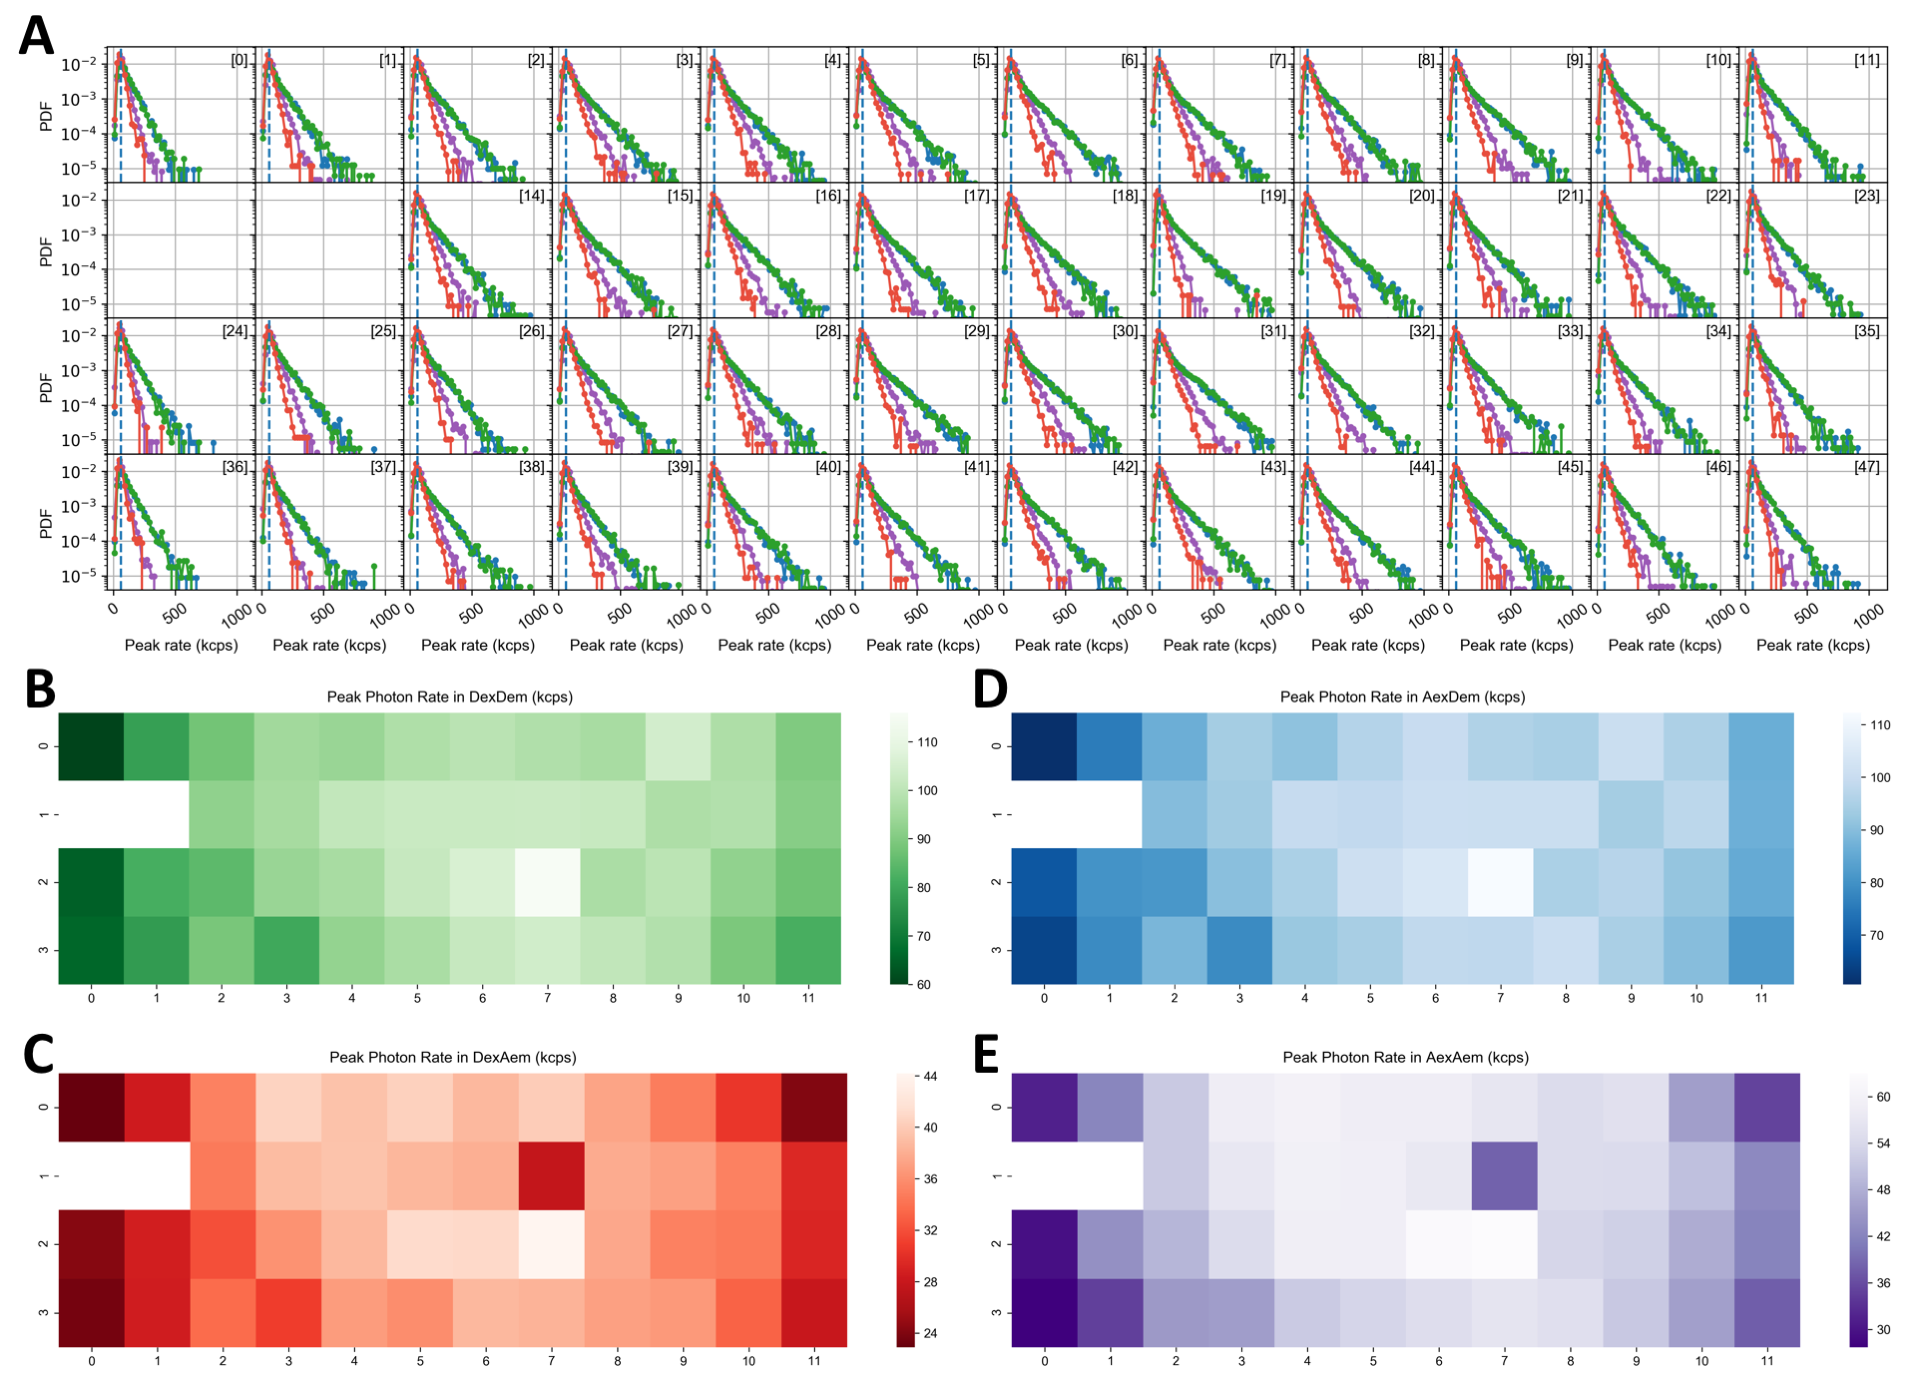
\includegraphics[width=0.9\textwidth]{{figures/2017-05-23_08_12d_phrates_summary}}
\caption{{\label{fig:pharates48_comp} Peak photon rate in each of the 48 spots for the 12
dsDNA sample. Panel A: full distribution of peak photon rates. Panels
B-E: Mean of the peak photon rate distribution in the different photon
steams. Color indicate different photon streams as follows: green
\(D_{ex}D_{em}\), red \(D_{ex}A_{em}\), light blue
\(DA_{ex}D_{em}\), purple \(DA_{ex}A_{em}\).%
}}
\end{figure*}

\begin{figure*}
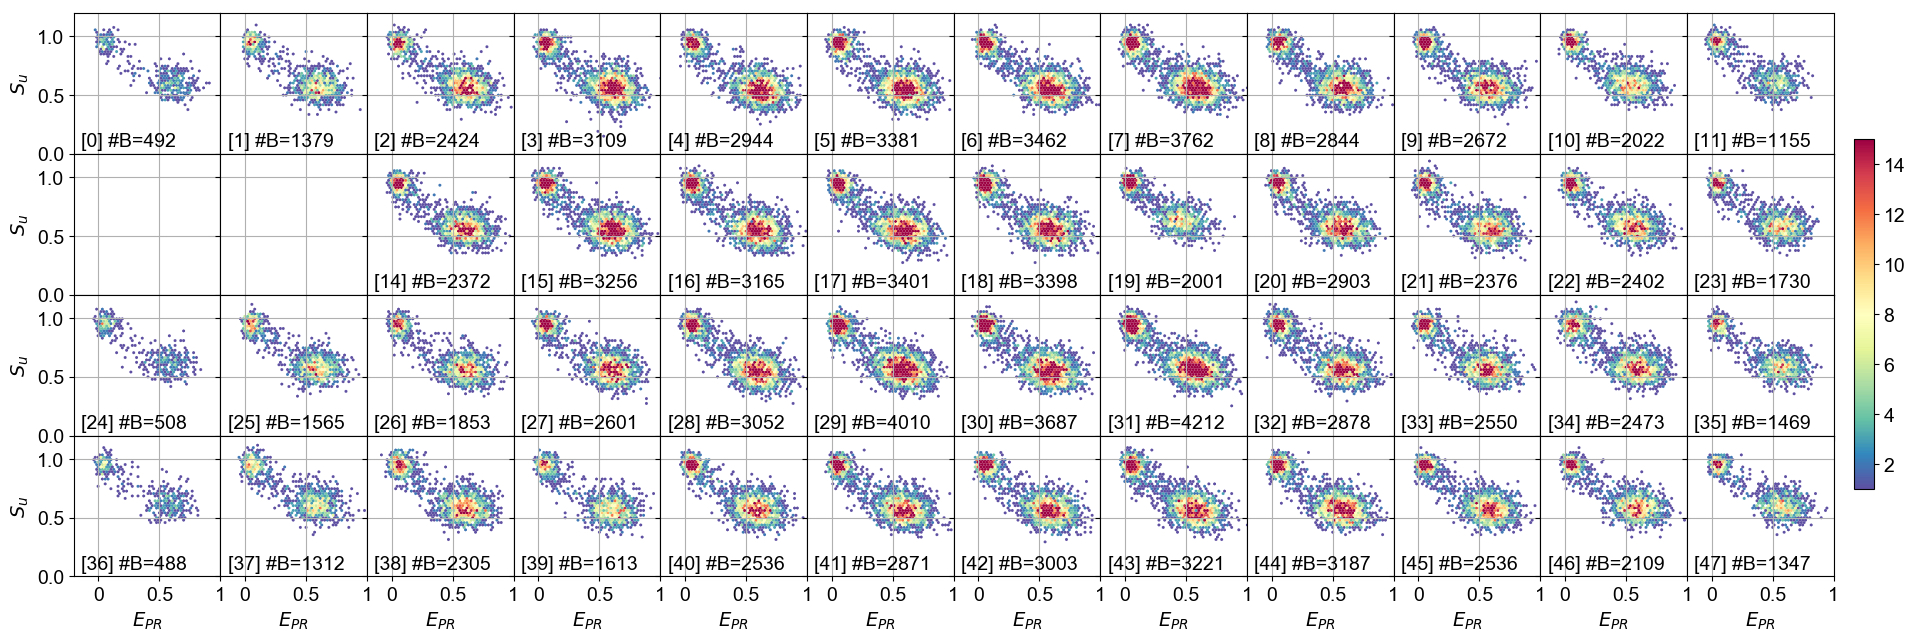
\includegraphics[width=0.9\textwidth]{{{figures/2017-05-23_08_12d_48spot_alex_hist_Su_all-bursts}}}
\caption{{\label{fig:alexhist48all} $E_{PR}$ versus $S_u$
histograms for the different spots for the 12d dsDNA sample. Two
populations visible D-only (cluster at \(E_{PR}=0\),
\(S_u=1\)) and FRET population (cluster at \(E_{PR}=0.6\),
\(S_u=0.6\)). Burst search is performed on all photons with
constant-threshold burst search (50~kcps). Burst selection is performed
on the total burst size after background correction with a threshold of
40 photons. Text in each subplot reports spot number
($[\cdot]$) and number of bursts (\#B).%
}}
\end{figure*}

\begin{figure*}
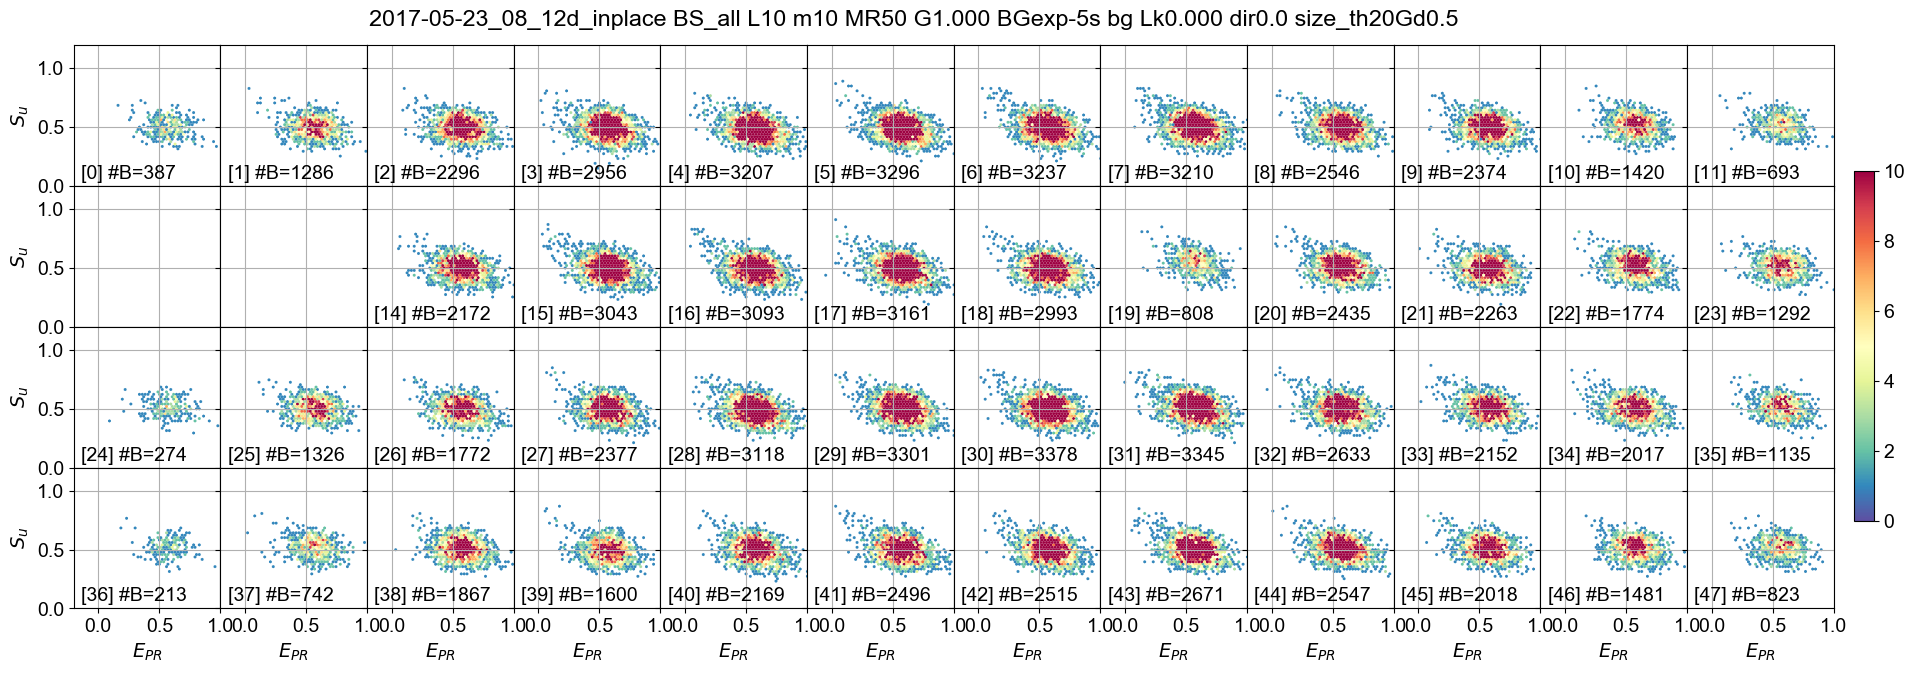
\includegraphics[width=0.9\textwidth]{{figures/2017-05-23_08_12d_48spot_alex_hist_Su_naa_AND_size_selection}}
\caption{{\label{fig:alexhist48fret} \(E_{PR}\) versus \(S_u\)
histograms for the different spots for the 12d dsDNA sample. Data and
burst search is identical as in figure~\ref{fig:alexhist48all}, while
burst selection has been tailored to select only the FRET population.
The burst selection criteria is the following: a burst is selected if
counts in \(D_{ex}DA_{em}\) stream are larger than 20 and counts in
\(DA_{ex}A_{em}\) stream are larger than 20. Text in each subplot
reports spot number ($[\cdot]$) and number of bursts (\#B).%
}}
\end{figure*}

\begin{figure}
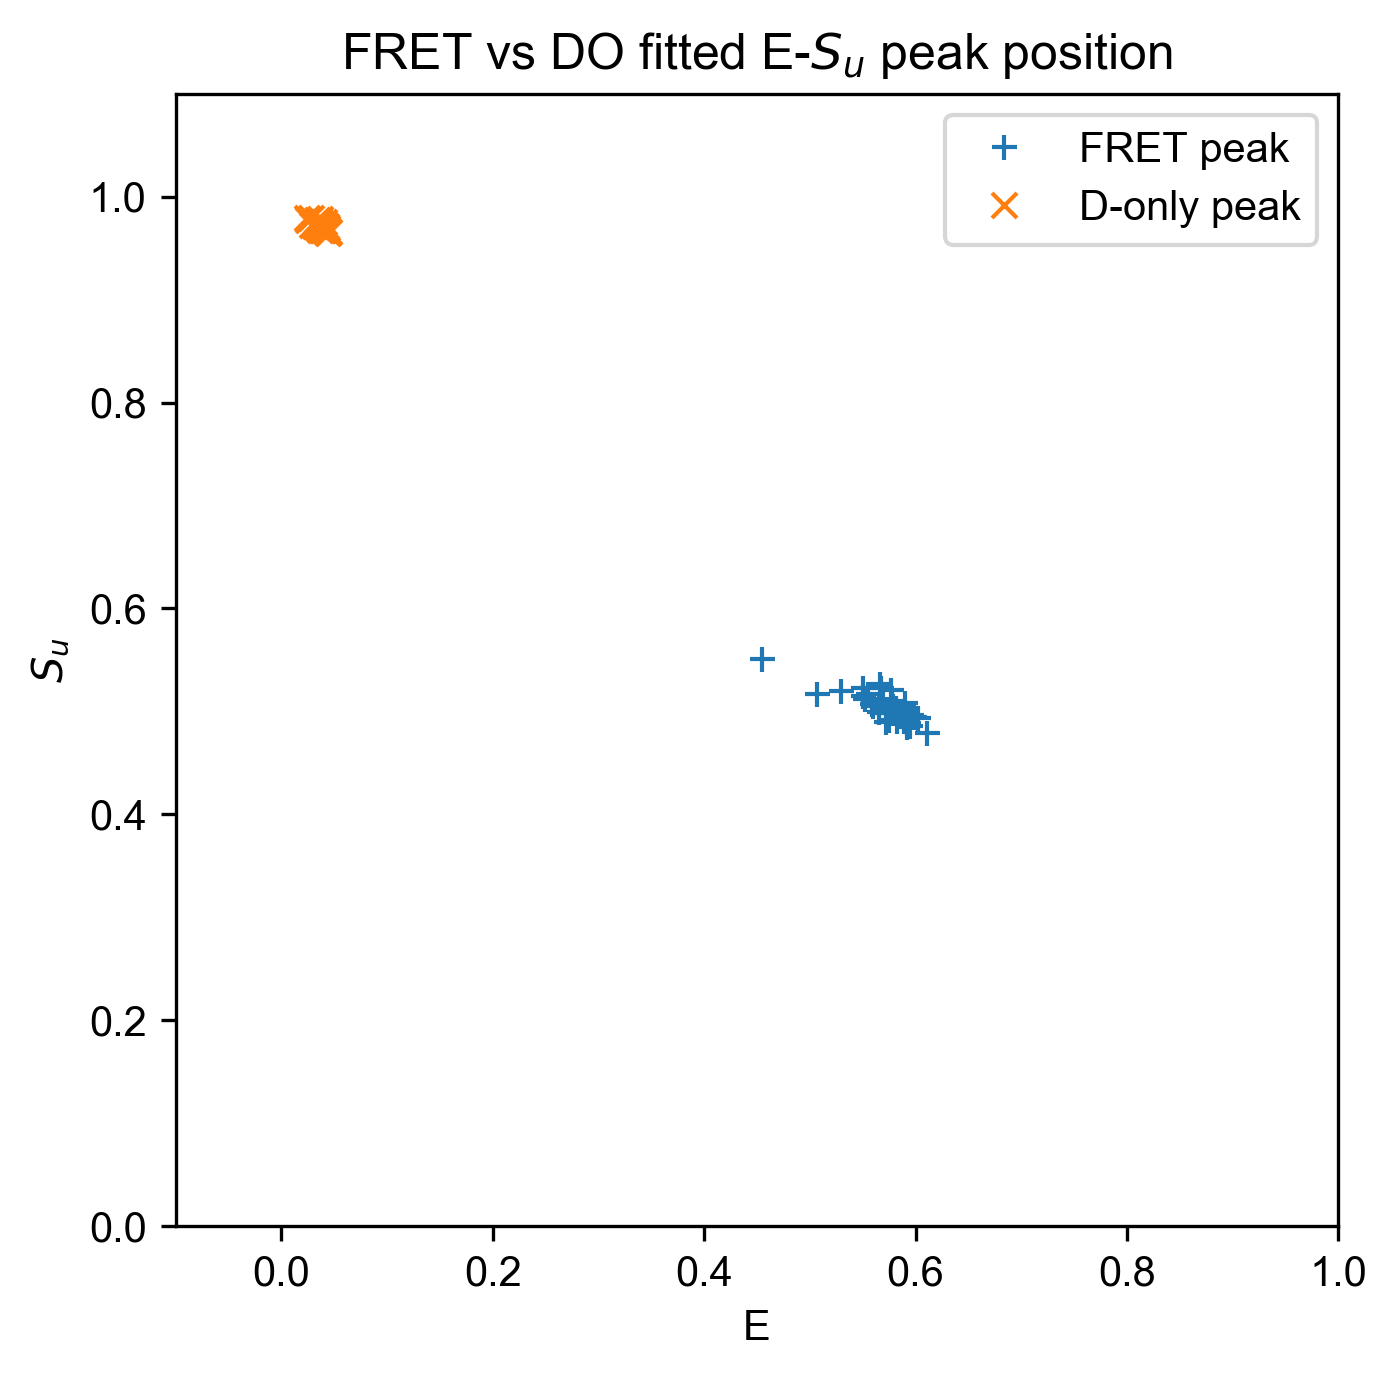
\includegraphics[width=0.7\columnwidth]{{figures/2017-05-23_08_12d_FRET_vs_DO_fitted_E-Su_peak_position}}
\caption{{\label{fig:fittedFRETscatter} Scatter plot of the fitted
$E_{PR}$, $S_u$ peak
position in the different spots for the D-only (\emph{orange cross})
and FRET population (\emph{blue plus}).}}
\end{figure}

\begin{figure*}
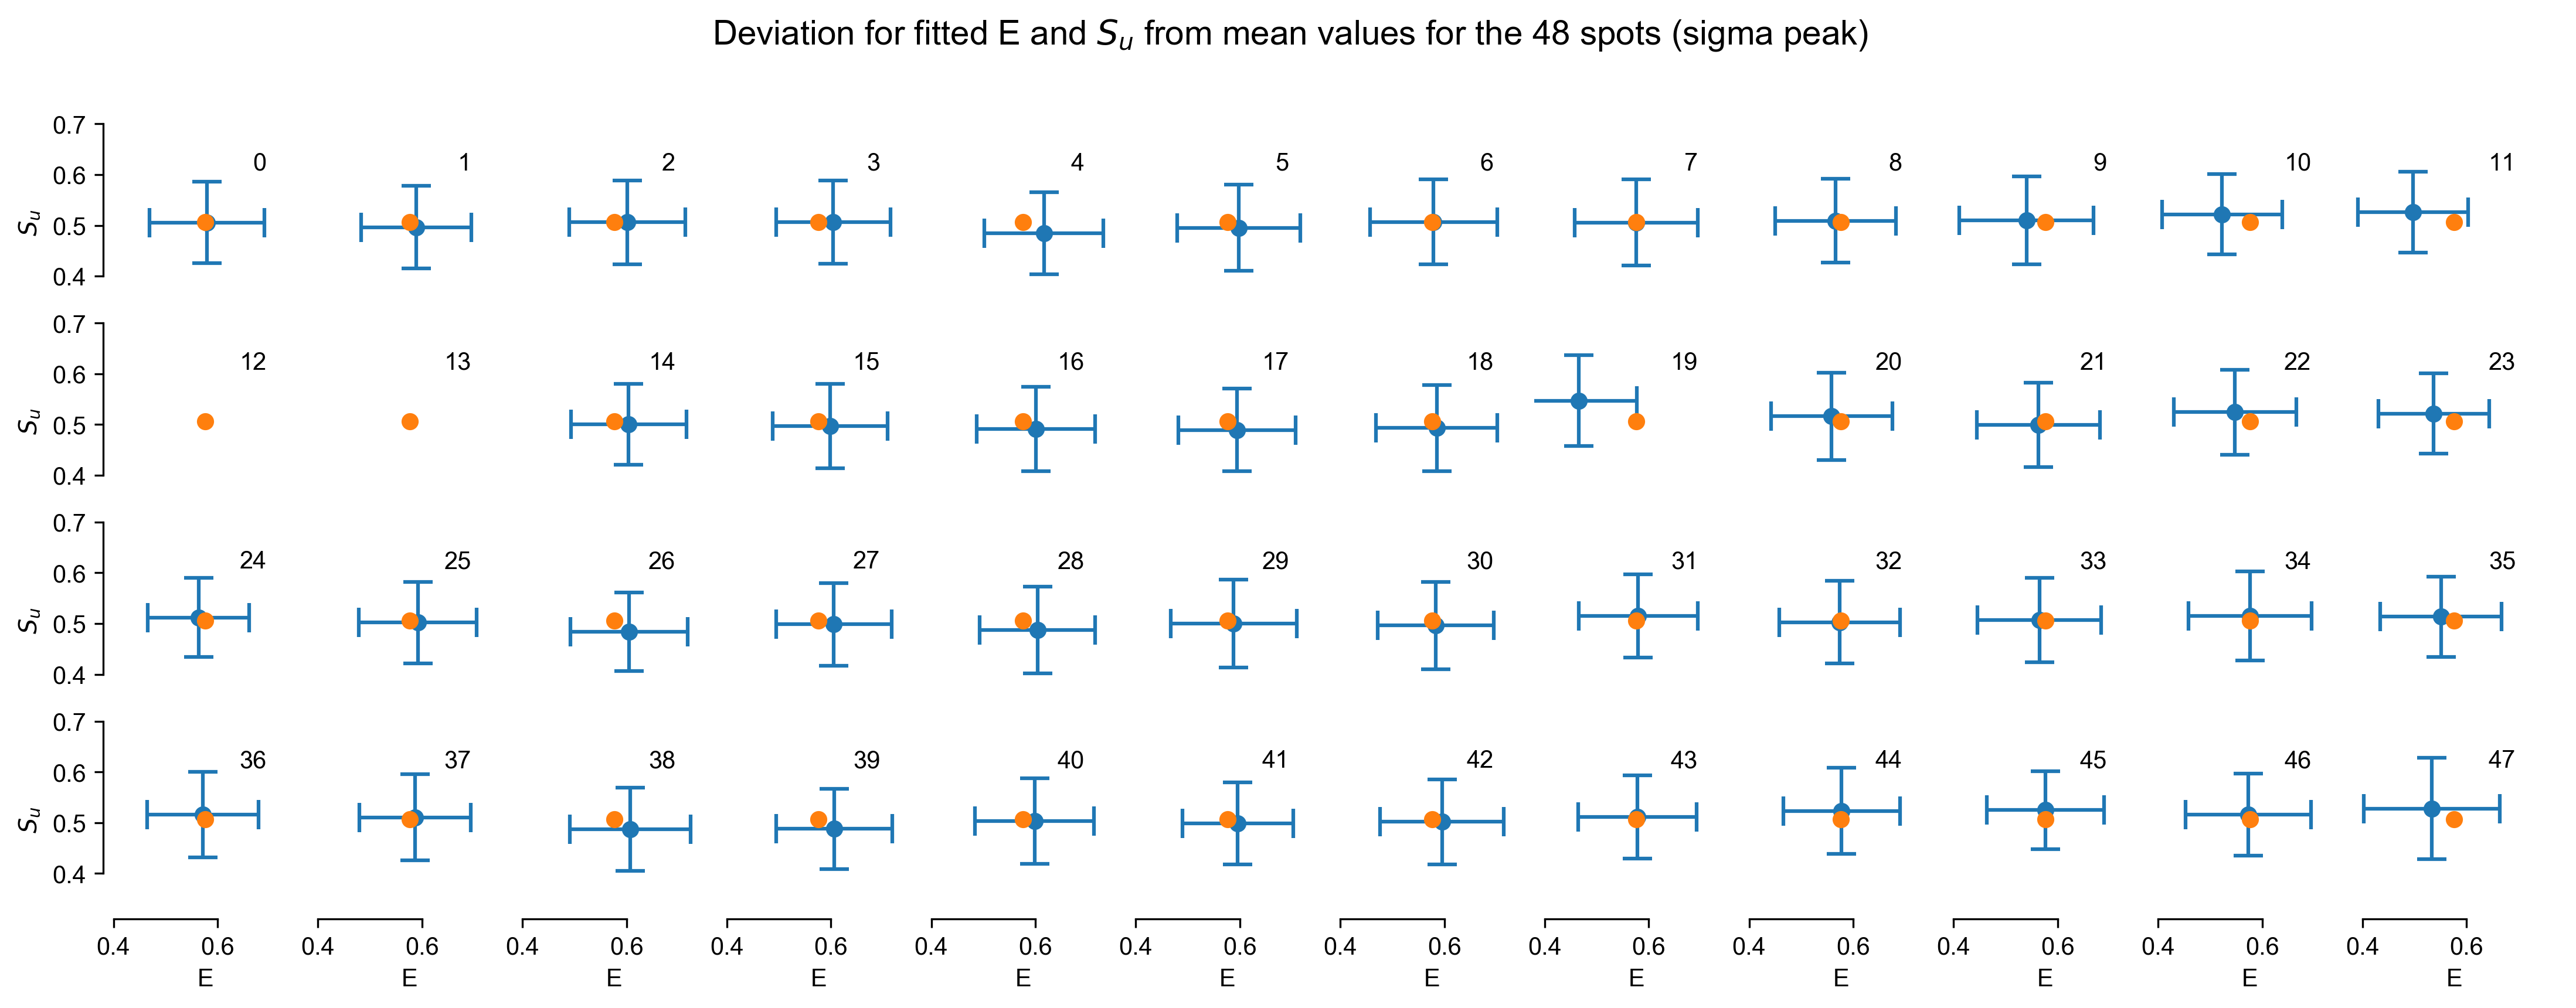
\includegraphics[width=0.9\textwidth]{{figures/2017-05-05_05_12d_48-spot_E-Su_peak_position_deviation_from_mean}}
\caption{{\label{fig:fretfit48vsmean} Fitted FRET peak position (\(E_{PR}, S_u\),
\emph{blue dots}) and \(\pm 1 \sigma \) of the fitted Gaussian
(\emph{blue error bars}) for the 48 spots. As a reference, the mean
\(E_{PR}, S_u\) across the 48 spots (\emph{orange dot}) is reported
in each subplot. The spot number is indicated in the top right corner of
each subplot.%
}}
\end{figure*}


\begin{acknowledgments}
We wish to acknowledge the support of the author community in using
REV\TeX{}, offering suggestions and encouragement, testing new versions,
\dots.
\end{acknowledgments}

\appendix
\section{Appendix: Alignment
Protocol}\label{appendix-alignment-protocol}

\subsection{Signal optimization for coarse alignment of LCOSs to
SPADs}

Signal is maximized by matching the center of the excitation pattern to
the center of the SPAD array. Figure XXX shows pixel map geometry for
both 12x4 SPAD arrays. The signal across top and bottom regions of the
detector is monitored in labview and the position of the LCOS excitation
pattern is adjusted with respect to the center position of the detector
to maximize the signal. This step allows coarse alignment of excitation
spots to SPADs by maximizing the LCOS-SPAD overlap.

\subsection{Coalignment of SPADs to LCOS pattern by
scanning}\label{coalignment-of-spads-to-lcos-pattern-by-scanning}

After green and red LCOS center positions are coarsely set during signal
optimization, both D and A detectors must be aligned with respect to the
LCOS excitation patterns. SPAD coalignment is achieved by matching SPAD
centers to LCOS centers with automated picomotor controllers (XXX,
reference picomotor control notebook). To this end, scans of center
pixels are collected and analyzed to determine the magnitude and
direction of movement required for alignment. The degree of overlap
between the excitation pattern and SPAD is quantified by a scanning
procedure where the detector is scanned with a 4x4 excitation pattern.
During a multispot scan, a 4x4 LCOS excitation pattern is used to scan
the center of the 12x4 pixel array by moving synchronously across the
4x4 center region in both X and Y directions (reference Appendix Figure
XXX). Scan results are monitored with the acquisition board and SPAD
counts from scanning with the 4x4 LCOS pattern are collected and plotted
against position (reference Appendix Figure XXX). Data from each spot is
fitted with a Gaussian in labview. The process of moving the detector
and scanning the resulting position is repeated until the center
position of the excitation pattern converges with the center position of
the detector to within 0.01 LCOS units.

In practice, alignment of both SPADs to excitation patterns requires
multiple steps. First the D-SPAD is scanned for precise location of
pixel centers using the reference green LCOS configuration from pattern
alignment. The 4x4 LCOS pattern is excited with the 532~nm laser and
excitation spots are used to scan the X and Y locations of pixels at the
center of the D-SPAD. The D-SPAD is moved in LCOS units to match the
center of the green LCOS. After each movement, scans are performed in
triplicate. This is repeated until convergence.

\subsection{Fine X-Y alignment of
SPADs}\label{fine-x-y-alignment-of-spads}

After alignment of the D-SPAD is fixed as previously described, the
A-SPAD is aligned to the D-SPAD by using the reference position of the
green LCOS under 532~nm illumination and moving the A-SPAD with picomotor
control. This step is repeated until center positions of the green LCOS
and A-SPAD converge. Once the centers are matched, the position of the
A-SPAD is fixed. The fixed center position of the A-SPAD is tested with
the red LCOS under 628~nm excitation, and the center location of the red
LCOS is adjusted to maximize overlap of both detectors. It is important
to note that due to spatial constraints the center position of the
A-SPAD can not be adjusted after it is aligned with respect to the green
LCOS, thus a mean position for the center of the red LCOS is selected
based on data from scan fits.

\subsection{X-Y pitch and rotation of green and red LCOSs by scan
fits}\label{x-y-pitch-and-rotation-of-green-and-red-lcoss-by-scan-fits}

Spot rotation and pitch must also be aligned for maximum overlap of
green and red excitation patterns. Alignment of rotation and pitch is an
iterative process that is achieved by calibration of rotation and pitch.
Calibration analysis with Alignment Summary (reference notebook and
supplementary figure showing rotation) is used to extract G and R LCOS
pitch and rotation parameters. Once parameters are determined more scan
are collected to test the quality of overlap between excitation
patterns.

After pitch and rotation of both excitation patterns converge, a final
fine alignment is achieved by matching the center position of the D-SPAD
the center of the green LCOS reference.

\section{Appendix: ALEX and PAX}
\label{sec:alex_pax}

In ALEX we have two alternation periods $D_{ex}$ and
$A_{ex}$ (respectively D or A excitation) and two
detectors (D and A). This results in four basic photon streams named
$D_{ex}D_{em}, D_{ex}A_{em}, A_{ex}D_{em}, A_{ex}A_{em}$.
The $A_{ex}D_{em}$ stream only contains
background because there is no fluorescent emission in the D spectral
band during A-laser excitation. For simplicity, we assume here and in
the following that all the quantities are corrected for
background\cite{Ingargiola_2016}.

A PAX setup has two detectors (D and A) but only one alternating laser (A).
We can still define two periods, one when only the D laser is on ($D_{ex}$)
and one when both lasers are on (${DA}_{ex}$).
As in ALEX, combining the two
excitation periods and the two detectors leads to four basic PAX
photon streams: $D_{ex}D_{em}, D_{ex}A_{em}, DA_{ex}D_{em}, A_{ex}A_{em}$.
Formally, the only difference
with the ALEX photon stream is that $A_{ex}$ in ALEX is
replaced with $DA_{ex}$ in PAX. Differently from ALEX, however,
all four photon streams in PAX contain useful fluorescent signal. In
particular, $DA_{ex}D_{em}$ contains D fluorescence due to D laser
excitation, while the corresponding term $A_{ex}D_{em}$ in ALEX
contains only background as noted before. With this notation, in both
ALEX and PAX, we can define the total signal during D excitation
(e.g.~burst size):

\begin{equation}
\Lambda = {F_{D_{ex}D_{em}} + F_{FRET}}
\label{eq:burstsize_raw}
\end{equation}

and the \(\gamma\) corrected version\cite{Lee_2005,Ingargiola_2016,Ingargiola_2017}:

\begin{equation}
\Lambda_\gamma = {\gamma\,F_{D_{ex}D_{em}} + F_{FRET}}
\label{eq:burstsize}
\end{equation}

where \(F_{FRET}\) is equal to \(F_{DexAem}\) after
D-leakage and A-direct-excitation corrections:

\begin{equation}
F_{FRET} = F_{D_{ex}A_{em}} - Lk\,F_{D_{ex}D_{em}} - Dir
\label{eq:F_FRET}
\end{equation}

With this definitions, we can write the proximity ratio
\(E_{PR}\) and FRET efficiency \(E\) expression
(valid for both ALEX and PAX):

\begin{equation}
E_{PR} = \frac{F_{FRET}}{\Lambda}
\label{eq:Epr}
\end{equation}

\begin{equation}
E = \frac{F_{FRET}}{\Lambda_\gamma}
\label{eq:E}
\end{equation}

While eq.~\ref{eq:Epr} and~\ref{eq:E} are exactly the same for both ALEX
and PAX, the \(S\) expression is slightly different. In
ALEX we define \(S\) as:

\begin{equation}
S = \frac{\Lambda}{\Lambda + F_{AexAem}}
\label{eq:S}
\end{equation}

and the corrected version \(S_{\gamma\beta}\) as:

\begin{equation}
S_{\gamma\beta} = \frac{\Lambda_\gamma}
{\Lambda_\gamma + \frac{F_{AexAem}}{\beta}}
\label{eq:Sgb}
\end{equation}

In PAX, we do not measure the \(F_{AexAem}\) stream, but we can
compute it as:

\begin{equation}
\tilde{F}_{AexAem} = F_{DAexAem} - F_{DexAem}
\label{eq:pax_Faa}
\end{equation}

Using eq.~\ref{eq:pax_Faa}, the expressions for \(S\) and
\(S_{\gamma\beta}\) become formally identical to eq.~\ref{eq:S} and
\ref{eq:Sgb} were the only difference is replacing \(F_{AexAem}\)
with \(\tilde{F}_{AexAem}\):

\begin{equation}
S = \frac{\Lambda}
{\Lambda + \tilde{F}_{AexAem}}
\label{eq:Spax}
\end{equation}

\begin{equation}
S_{\gamma\beta} = \frac{\Lambda_\gamma}
{\Lambda_\gamma + \frac{\tilde{F}_{AexAem}}{\beta}}
\label{eq:Sgb_pax}
\end{equation}

In PAX we can take advantage of the additional signal in
\(F_{AexDem}\) and derive an equivalent set of PAX-enhanced
expressions for \(E\) and \(S\). We can
start extending the definitions of the total FRET signal of
eq.~\ref{eq:burstsize_raw} and~\ref{eq:burstsize} by including
\(F_{AexDem}\) as follows:

\begin{equation}
\Lambda_{PAX} = {F_{DexDem} + F_{AexDem} + 2 F_{FRET}}
\label{eq:burstsizerawpaxe}
\end{equation}

\begin{equation}
\Lambda_{\gamma,PAX} = {\gamma\,(F_{DexDem} + F_{AexDem}) + 2 F_{FRET}}
\label{eq:burstsize_paxe}
\end{equation}

Based on eq.~\ref{eq:burstsizerawpaxe} and \ref{eq:burstsize_paxe}, we
can write PAX-enhanced expressions for \(E\) and
\(S\):

\begin{equation}
E_{PR,PAX} = \frac{2\,F_{FRET}}
{\Lambda_{PAX}}
\label{eq:Epr_paxe}
\end{equation}

\begin{equation}
E_{PAX} = \frac{2\,F_{FRET}}
{\Lambda_{\gamma,PAX}}
\label{eq:Epaxe}
\end{equation}

\begin{equation}
S = \frac{\Lambda_{PAX}}
{\Lambda_{PAX} + \tilde{F}_{AexAem}}
\label{eq:Spaxe}
\end{equation}

\begin{equation}
S_{\gamma\beta,PAX} = \frac{\Lambda_{\gamma,PAX}}
{\Lambda_{\gamma,PAX} + \frac{2\tilde{F}_{AexAem}}{\beta}}
\label{eq:Sgb_paxe}
\end{equation}


Eq.~\ref{eq:Epr_paxe}, \ref{eq:Epaxe}, \ref{eq:Spaxe}
and~\ref{eq:Sgb_paxe} contain more photons than the classical expressions
and therefore should result in lower shot-noise. However this effect is
mitigated by the fact that \(F_{FRET}\) is counted twice (to
compensate for the doubling of the D signal) and therefore its
shot-noise is amplified.


\subsection{Modified stoichiometry}\label{modified-stoichiometry}

By replacing \(\tilde{F}_{AexAem}\) with \(F_{AexDAem}\) in eq.
\ref{eq:Spax}, we can define a modified stoichiometry \(S_u\)
as follows

\begin{equation}
S_u = \frac{\Lambda}
{\Lambda + F_{AexDAem}}
\label{eq:Su}
\end{equation}

This expression avoids the subtraction of photon counts necessary to
compute \(\tilde{F}_{AexAem}\) in PAX (eq.~\ref{eq:pax_Faa}) and the
corresponding increase in shot-noise. As a results, the
\(S_u\) distributions are tighter and permit easier
separation of FRET and D-only population, which is the main purpose of
\(S\). Note, however, that \(S_u\) has a
built-in dependency on the population FRET value, in particular
\(S_u\) decreases with the increasing \(E\).
Nonetheless, even at low FRET values, better separation between FRET and
D-only population was achieved using \(S_u\) instead of
\(S\). In principle, once populations are separated, one
can return to use the classical \(S\) expression for the
purpose of computing gamma factors. Our interest, in the current paper,
was not recovering absolute FRET values and D-A distances, but rather
demonstrating the capabilities of the smFRET-PAX system in terms of
spot-uniformity and throughput increase. Therefore, we did not compute a
complete gamma factor calibration. However, we addressed the differences
in collection and detection efficiency across the different spots using
a ``relative'' gamma coefficient \(\chi_{ch}\) as illustrated in
section \ref{sec:perchcorr}.


\section{Per channel corrections}

\label{sec:perchcorr}

\subsection{Gamma correction}

The gamma-factor of each channel \(\gamma_{ch}\) can be factorized in
an average factor \(\gamma_m\) and a spot-specific adjustment
\(\chi_{ch}\):

\begin{equation}
\gamma_{ch} = \gamma_m \cdot \chi_{ch}
\label{eq:gamma_split}
\end{equation}

The factor \(\chi_{ch}\) can be easily computed from measurable
quantities according to the following expression:

\begin{equation}
\chi_{ch} = \frac{\frac{1}{\langle E_{PR\,ch} \rangle_{ch}} - 1}{\frac{1}{E_{PR\,ch}} - 1}
\label{eq:chich}
\end{equation}

In eq.~\ref{eq:chich}, \(E_{PR\,ch}\) is the population-level
proximity ratio for a specific channel, and \( \langle E_{PRch} \rangle_{ch} \) is the
mean of these proximity ratios across all the \(N\)
channels (in this case \(N= 48\)).

The derivation of eq.~\ref{eq:chich} is straightforward and is reported
below. We start from the well known relation between \(E\)
and \(E_{PR}\) when only \(\gamma\) correction is
considered:

\begin{equation}
E = \frac{1}{1 + \gamma \left( \frac{1}{E_{PR}} - 1 \right)}
\label{eq:EfuncEpr}
\end{equation}

Inverting eq.~\ref{eq:EfuncEpr} we obtain:

\begin{equation}
\gamma = \frac{\frac{1}{E} - 1}{\frac{1}{E_{PR}} - 1}
\label{eq:gamma_funcEEpr}
\end{equation}

Formally, we can define \(\gamma = \gamma_1 \gamma_2 \) and a partially corrected
proximity ratio \(E_1\) as:

\begin{equation}
E_1 = \frac{1}{1 + \gamma_1 \left( \frac{1}{E_{PR}} - 1 \right)}
\end{equation}

Then, we can express \(E\) as a function of the partially
corrected \(E_{1}\) by a simple substitution of
\ref{eq:gamma_funcEEpr} into eq.~\ref{eq:EfuncEpr}:

\begin{equation}
E = \frac{1}{1 + \gamma_2 \left( \frac{1}{E_1} - 1 \right)}
\label{eq:EfuncE1}
\end{equation}

Eq.~\ref{eq:EfuncE1} shows that gamma corrections are composable. In the
multispot case, we apply this property to split the gamma correction in
a spot-specific correction and in an average correction as in
\ref{eq:gamma_split}. Therefore, eq.~\ref{eq:chich} directly derives
from \ref{eq:gamma_funcEEpr} with simple substitutions.

\subsection{Beta correction}

Since, formally eq.~\ref{eq:S} and~\ref{eq:Sgb} have the same form of
\(E_{PR}\) and \(E\), we can write an expression
equivalent to \ref{eq:EfuncEpr} for \(S\) and
\(S_{\gamma\beta}\). Dropping the \(\gamma\) subscript, we
obtain:

\begin{equation}
S_{\beta} = \frac{1}{1 + \frac{1}{\beta} \left( \frac{1}{S} - 1 \right)}
\label{eq:SbfuncS}
\end{equation}

Following the same arguments as in previous section, we can factorize
the beta correction in a spot-average \(\beta_m\) and a
per-channel correction \(\beta_{ch}\) as follows:

\begin{equation}
\beta = \beta_m \, \beta_{ch}
\label{eq:beta_factor}
\end{equation}

Analogously to eq.~\ref{eq:chich}, we can compute \(\beta_{ch}\) as:

\begin{equation}
\frac{1}{\beta_{ch}} = \frac{\frac{1}{\langle S_{ch} \rangle_{ch}} - 1}{\frac{1}{S_{ch}} - 1}
\label{eq:betach}
\end{equation}

where \(S_{ch}\) is the population-level non-beta-corrected
stoichiometry for a specific channel, and \( \langle S_{ch} \rangle_{ch} \) is the
mean of these stoichiometry across all the $N$
channels ($N= 48$ in this case).


\nocite{*}
\bibliography{biblio}% Produces the bibliography via BibTeX.

\end{document}
%
% ****** End of file aipsamp.tex ******
